% rotate-cyclic-n9-l6.tex

\documentclass[tikz]{standalone}
\usetikzlibrary{shapes.multipart, positioning}

\begin{document}
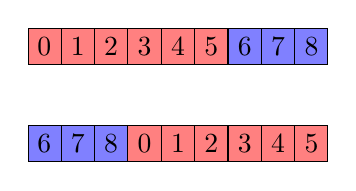
\begin{tikzpicture}[array/.style = {
    rectangle split, rectangle split parts = #1, 
    rectangle split horizontal, 
    rectangle split part fill = {red!50, red!50, red!50, red!50, red!50, red!50, blue!50},
    draw, anchor = center, minimum width = 0.60cm}]
  \node (a) [array = 9] 
  {0\nodepart{two}1\nodepart{three}2\nodepart{four}3\nodepart{five}4\nodepart{six}5\nodepart{seven}6\nodepart{eight}7\nodepart{nine}8};

  \node [array = 9, below = of a.center,
    rectangle split part fill = {blue!50, blue!50, blue!50, red!50}] 
  {6\nodepart{two}7\nodepart{three}8\nodepart{four}0\nodepart{five}1\nodepart{six}2\nodepart{seven}3\nodepart{eight}4\nodepart{nine}5};
\end{tikzpicture}
\end{document}